\subsection{DB Implementering}

Til implementering og håndtering af databasen i .NET har gruppen valgt at benytte Entity framework core.
EF core gør det nemt at oprette og håndtere objekter C\# som skal gemmes eller hentes i databasen.\\
Til modellering af databasen benyttes det udarbejde ER-diagram hvorpå keys og relations er bestemt.\\
Disse keys og relations opsættes i projektets backend ved hjælp af fluent api, hvori man nemt kan specificere keys, foreign keys, relations, hasData og meget mere.\\
Ved ændringer af databasens udseende og form kan EFcore migrations hjælpe med at oprette de korrekte queries således at databasen bliver ændret korrekt, samt at man ved forkerte ændringer hurtigt kan hoppe tilbage til en tidligere migration ved eventuelle fejl. I EF core benyttes Language Integrated Query (LINQ) til at skrive ensartede queries til databasen.\\

Der er i projektets backend oprettet klasser, models, tilsvarende ER diagrammernes entiteter. Udover det valgte atributter er der også oprettet navigationals i de nødvendige klasse så der kan laves relationer.
På figur xx herunder ses opsætningen af keys for de forskellige entiteter. Disse er opsat med fluent api efter ER diagrammerne på figur xx og xx.

\begin{figure}[H]
\centering
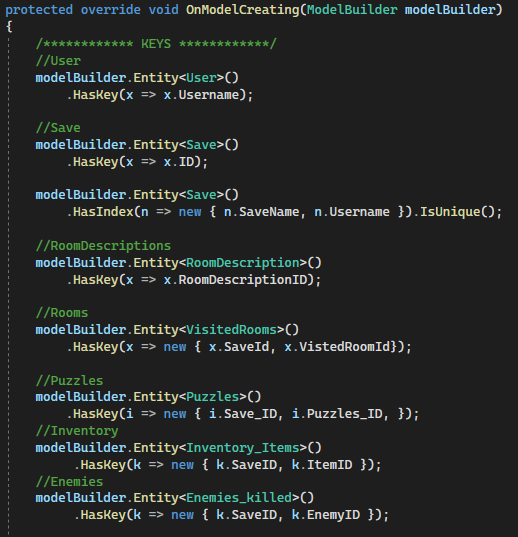
\includegraphics[width = 0.7\textwidth]{02-Body/Images/DAL-Database/DbKeys.PNG}
\caption{Opsætning af keys og unikke indexes for de forskellige entiteter i backends DbContext}
\label{fig:DbKeys}
\end{figure}

Udover de forskellige keys, skal der også opsætte relationer mellem de forskellige entiteter, som vist på ER-Diagrammerne \autoref{fig:ER-Roomdescription} og \autoref{fig:ER-GameSave}, samt referencer til foreign keys. 
Opsætningen kan ses på \autoref{fig:DbRelations} herunder: 

\begin{figure}[H]
\centering
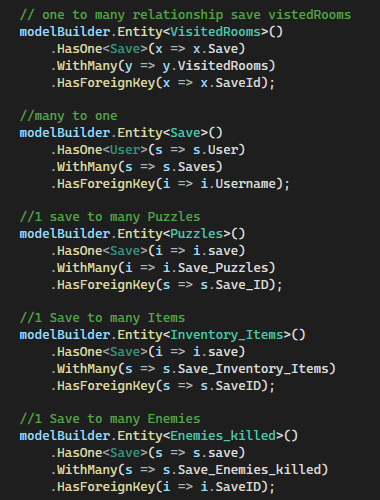
\includegraphics[width = 0.5\textwidth]{02-Body/Images/DAL-Database/DbRelations.PNG}
\caption{Opsætning af relations og foreign keys for de forskellige entiteter i backends DbContext}
\label{fig:DbRelations}
\end{figure}

Databasen er seedet ved hjælp af hasdata funktionen. Her oprettes en enkelt bruger, ”Gamer1”, med password ”123”, som hashes ind i databasen. "Gamer1" får derudover også 5 tilhørende "tomme" saves og til slut er der også indsat rumbeskrivelser for hver af de 20 rum. Dette ses på \autoref{fig:DbSeeding} herunder.

\begin{figure}[H]
\centering
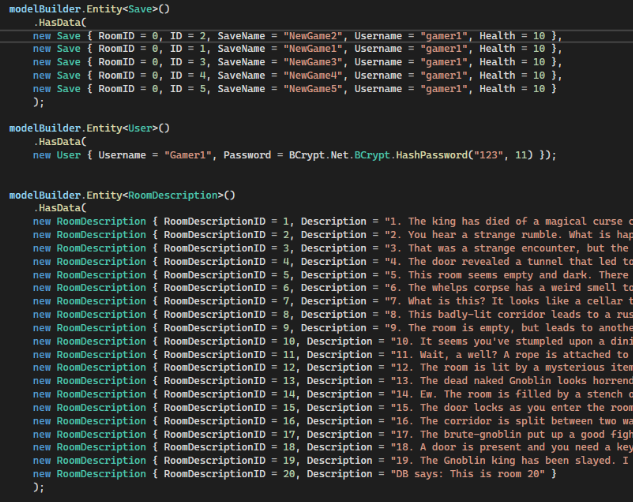
\includegraphics[width = 0.85\textwidth]{02-Body/Images/DAL-Database/DbSeeding.PNG}
\caption{Seeding af databasen med en enkel bruger, "Gamer1", 5 tilhørende "tomme" saves og beskrivelser af historien til de 20 forskellige rum}
\label{fig:DbSeeding}
\end{figure}